% Template for ICASSP-2021 paper; to be used with:
%          spconf.sty  - ICASSP/ICIP LaTeX style file, and
%          IEEEbib.bst - IEEE bibliography style file.
% --------------------------------------------------------------------------
\documentclass{article}
\usepackage{spconf,amsmath,graphicx}
\usepackage{hyperref}

% Example definitions.
% --------------------
\def\x{{\mathbf x}}
\def\L{{\cal L}}

% Title.
% ------
\title{Ze Awesome French Audio Researcher (ZAFAR)}
%
% Single address.
% ---------------
\name{Zafar Rafii}
\address{PhD in Electrical Engineering \& Computer Science \\
\texttt{zafarrafii@gmail.com}}
%
% For example:
% ------------
%\address{School\\
%	Department\\
%	Address}
%
% Two addresses (uncomment and modify for two-address case).
% ----------------------------------------------------------
%\twoauthors
%  {A. Author-one, B. Author-two\sthanks{Thanks to XYZ agency for funding.}}
%	{School A-B\\
%	Department A-B\\
%	Address A-B}
%  {C. Author-three, D. Author-four\sthanks{The fourth author performed the work
%	while at ...}}
%	{School C-D\\
%	Department C-D\\
%	Address C-D}
%
\begin{document}
%\ninept
%
\maketitle
%
\begin{abstract}
We present Zafar, Ze Awesome French Audio Researcher. The proposed researcher has a PhD in electrical engineering and computer science from Northwestern University, with a focus on audio signal analysis. He has over 30 publications, including conference papers, journal articles, and patents, with 1,500 citations overall. He is actively involved within the research community, as a reviewer for numerous conferences and journals, a member of the IEEE audio and acoustic signal processing technical committee, and an organizer of networking meetups in the San Francisco Bay Area. He is currently a research engineer manager at Gracenote, where he is working on a number of projects involving, among others, audio recognition, audio separation, and audio classification.
\end{abstract}
%
\begin{keywords}
Research, audio, signal processing, separation, recognition, classification
\end{keywords}
%
\section{Introduction}
\label{sec:intro}

The proposed researcher is named Zafar Rafii. He received a PhD in electrical engineering and computer science from \href{https://www.northwestern.edu/}{Northwestern University} in 2014. He was with the \href{https://interactiveaudiolab.github.io/}{Interactive Audio Lab}, under the supervision of professor Bryan Pardo. Before that, he was a research engineer at Audionamix, in France. He is now a research engineer manager in the audio group of the Applied Research group at \href{https://www.gracenote.com/}{Gracenote}.

\begin{figure}[htb]
\centering
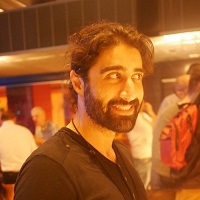
\includegraphics[width=0.5\columnwidth]{zafar.jpg}
\caption{Overview of the proposed researcher.}
\label{fig:res}
\end{figure}

The proposed researcher has interest and expertise in audio signal analysis; he has worked on a number of projects, including:
\begin{itemize}
\setlength\itemsep{-0.5em}
\item Blind source separation
\item Spatial source separation
\item Digital audio effects
\item Audio fingerprinting
\item Cover song identification
\item Audio encoding analysis
\item Audio beamforming
\item Audio watermarking
\item Audio/video segmentation
\item Audio classification
\end{itemize}


\section{MAJOR HEADINGS}
\label{sec:majhead}

Major headings, for example, "1. Introduction", should appear in all capital
letters, bold face if possible, centered in the column, with one blank line
before, and one blank line after. Use a period (".") after the heading number,
not a colon.

\subsection{Subheadings}
\label{ssec:subhead}

Subheadings should appear in lower case (initial word capitalized) in
boldface.  They should start at the left margin on a separate line.
 
\subsubsection{Sub-subheadings}
\label{sssec:subsubhead}

Sub-subheadings, as in this paragraph, are discouraged. However, if you
must use them, they should appear in lower case (initial word
capitalized) and start at the left margin on a separate line, with paragraph
text beginning on the following line.  They should be in italics.

\section{PRINTING YOUR PAPER}
\label{sec:print}

Print your properly formatted text on high-quality, 8.5 x 11-inch white printer
paper. A4 paper is also acceptable, but please leave the extra 0.5 inch (12 mm)
empty at the BOTTOM of the page and follow the top and left margins as
specified.  If the last page of your paper is only partially filled, arrange
the columns so that they are evenly balanced if possible, rather than having
one long column.

In LaTeX, to start a new column (but not a new page) and help balance the
last-page column lengths, you can use the command ``$\backslash$pagebreak'' as
demonstrated on this page (see the LaTeX source below).

\section{PAGE NUMBERING}
\label{sec:page}

Please do {\bf not} paginate your paper.  Page numbers, session numbers, and
conference identification will be inserted when the paper is included in the
proceedings.

\section{ILLUSTRATIONS, GRAPHS, AND PHOTOGRAPHS}
\label{sec:illust}

Illustrations must appear within the designated margins.  They may span the two
columns.  If possible, position illustrations at the top of columns, rather
than in the middle or at the bottom.  Caption and number every illustration.
All halftone illustrations must be clear black and white prints.  Colors may be
used, but they should be selected so as to be readable when printed on a
black-only printer.

Since there are many ways, often incompatible, of including images (e.g., with
experimental results) in a LaTeX document, below is an example of how to do
this \cite{Lamp86}.

\section{FOOTNOTES}
\label{sec:foot}

Use footnotes sparingly (or not at all!) and place them at the bottom of the
column on the page on which they are referenced. Use Times 9-point type,
single-spaced. To help your readers, avoid using footnotes altogether and
include necessary peripheral observations in the text (within parentheses, if
you prefer, as in this sentence).

% Below is an example of how to insert images. Delete the ``\vspace'' line,
% uncomment the preceding line ``\centerline...'' and replace ``imageX.ps''
% with a suitable PostScript file name.
% -------------------------------------------------------------------------
\begin{figure}[htb]

\begin{minipage}[b]{1.0\linewidth}
  \centering
  \centerline{\includegraphics[width=8.5cm]{image1}}
%  \vspace{2.0cm}
  \centerline{(a) Result 1}\medskip
\end{minipage}
%
\begin{minipage}[b]{.48\linewidth}
  \centering
  \centerline{\includegraphics[width=4.0cm]{image3}}
%  \vspace{1.5cm}
  \centerline{(b) Results 3}\medskip
\end{minipage}
\hfill
\begin{minipage}[b]{0.48\linewidth}
  \centering
  \centerline{\includegraphics[width=4.0cm]{image4}}
%  \vspace{1.5cm}
  \centerline{(c) Result 4}\medskip
\end{minipage}
%
\caption{Example of placing a figure with experimental results.}
\label{fig:res}
%
\end{figure}


% To start a new column (but not a new page) and help balance the last-page
% column length use \vfill\pagebreak.
% -------------------------------------------------------------------------
%\vfill
%\pagebreak

\section{COPYRIGHT FORMS}
\label{sec:copyright}

You must submit your fully completed, signed IEEE electronic copyright release
form when you submit your paper. We {\bf must} have this form before your paper
can be published in the proceedings.

\section{RELATION TO PRIOR WORK}
\label{sec:prior}

The text of the paper should contain discussions on how the paper's
contributions are related to prior work in the field. It is important
to put new work in  context, to give credit to foundational work, and
to provide details associated with the previous work that have appeared
in the literature. This discussion may be a separate, numbered section
or it may appear elsewhere in the body of the manuscript, but it must
be present.

You should differentiate what is new and how your work expands on
or takes a different path from the prior studies. An example might
read something to the effect: "The work presented here has focused
on the formulation of the ABC algorithm, which takes advantage of
non-uniform time-frequency domain analysis of data. The work by
Smith and Cohen \cite{Lamp86} considers only fixed time-domain analysis and
the work by Jones et al \cite{C2} takes a different approach based on
fixed frequency partitioning. While the present study is related
to recent approaches in time-frequency analysis [3-5], it capitalizes
on a new feature space, which was not considered in these earlier
studies."

\vfill\pagebreak

\section{REFERENCES}
\label{sec:refs}

List and number all bibliographical references at the end of the
paper. The references can be numbered in alphabetic order or in
order of appearance in the document. When referring to them in
the text, type the corresponding reference number in square
brackets as shown at the end of this sentence \cite{C2}. An
additional final page (the fifth page, in most cases) is
allowed, but must contain only references to the prior
literature.

% References should be produced using the bibtex program from suitable
% BiBTeX files (here: strings, refs, manuals). The IEEEbib.bst bibliography
% style file from IEEE produces unsorted bibliography list.
% -------------------------------------------------------------------------
\bibliographystyle{IEEEbib}
\bibliography{strings,refs}

\end{document}
